\documentclass[10pt,twocolumn,a4paper]{article}

\usepackage[margin=1.65cm]{geometry}
\usepackage{graphicx}
\usepackage{amsmath}
\usepackage{amssymb}
\usepackage{booktabs}
\usepackage{hyperref}

\title{\textbf{Logarithmic Oscillatory Dark Energy: Official DESI DR2 BAO, DES-SN5YR Dovekie, and Full 3D Planck Constraints with Pre-Registered 2027 Euclid Anisotropic Forecasts}}

\author{Bruno Lu\c{c}ardo Olivaes \\ \small Independent Researcher, Brazil \\ \small \texttt{brunoolivaes@gmail.com} $\cdot$ ORCID: \href{https://orcid.org/0009-0003-5351-446X}{0009-0003-5351-446X}}

\date{November 2026}

\begin{document}

\twocolumn[{%
  \begin{@twocolumnfalse}
    \maketitle
    \begin{abstract}
    \noindent Standard Chevallier--Polarski--Linder (CPL) parameterizations of dynamical dark energy ($w(a) = w_0 + w_a(1-a)$) extrapolate monotonically into deep phantom regimes as $z \to \infty$. We investigate a bounded, scale-invariant logarithmic harmonic alternative, $w(a) = -1 + A\sin\!\left(\frac{2\pi}{\lambda}\ln a + \phi_0\right)$, for which the relativistic continuity equation admits an exact closed-form dark energy density $\rho_{\mathrm{DE}}(z)$. In this Version~3.0 stress-audit ahead of ESA Euclid Data Release~1 (mid-2027), we upgrade our full-covariance likelihood engine to ingest: (1)~both the uncalibrated Pantheon+ compilation ($N = 1,580$) and the official DES-SN5YR Dovekie Hubble-diagram compilation ($N = 1,820$) using full statistical-plus-systematic inverse covariances; (2)~official DESI DR2 Baryon Acoustic Oscillation (BAO) measurements (arXiv:2503.14738, $N = 13$ observables across $0.295 \le z \le 2.330$); and (3)~the full 3D Planck~2018 CMB distance prior $\mathbf{v}_{\mathrm{CMB}} = (R, l_A, \omega_b)$ with correlated $3\times 3$ covariance. Across six independent stress tests, we prove three decisive results. First, replacing 1D Planck~$R$ with full 3D Planck shifts $\Delta\chi^2_{\mathrm{CPL}}$ on Pantheon+ + DESI DR1 from $-3.76$ to $-6.03$, while with DESI DR2 the preference reaches $\Delta\chi^2 = -7.43$ (CPL) / $-8.05$ (\texttt{OSC\_CS}) using Pantheon+ and $\Delta\chi^2 = -10.31$ (CPL, $\Delta\mathrm{AIC}=-6.31$) / $-10.52$ (\texttt{OSC\_CS}, $\Delta\mathrm{AIC}=-4.52$) using DES-SN5YR Dovekie. Second, a $N_{\mathrm{MC}} = 2,000$ parametric bootstrap Look-Elsewhere periodogram across $\lambda \in [0.8, 12.0]$ finds $N_{\mathrm{eff}} = 1.633\text{--}1.976$ effective trials, correcting local significance from $2.37\sigma \to 2.18\sigma$ ($p_{\mathrm{global}} = 0.0292$, Pantheon+ + DR2) and $2.80\sigma \to 2.57\sigma$ ($p_{\mathrm{global}} = 0.0102$, DES-SN5YR + DR2), while proving that \texttt{OSC\_CS} improves over CPL by only $\Delta\chi^2 = +0.21\text{--}+0.62$ because long-wavelength harmonics ($\lambda \to 12$) geometrically mimic CPL at $z \lesssim 2$. Third, slope-decoupled orthogonal $(C, S)$ Ensemble MCMC (incorporating the exact polar Jacobian $+\ln(\lambda/2\pi)$) achieves $\hat{R}_{\mathrm{split}} \le 1.116$ ($\mathrm{ESS}_{\min} \ge 1,294$), yielding $A = 0.536^{+0.265}_{-0.245}$ ($95\%$ upper limit $A_{95} = 0.925$, DES-SN5YR + DR2). Finally, replacing 1D $H(z)$ forecasts with a coupled anisotropic $(D_M/r_d, H r_d)$ Fisher matrix shows that Euclid DR1-2027 (with external DES-SN5YR+DR2+CMB prior) reaches $A_{3\sigma} \approx 0.167\text{--}0.206$ (full survey: $0.069\text{--}0.086$) across $\lambda \in [2.1, 12.0]$, and we publish pre-registered blind 2027 Euclid BAO predictions across $z \in \{1.00, 1.20, 1.40, 1.65\}$.
    \end{abstract}
    \vspace{0.45cm}
  \end{@twocolumnfalse}
}]

\section{Introduction and Evolution (v1.0 to v3.0)}
Recent Baryon Acoustic Oscillation (BAO) measurements from the Dark Energy Spectroscopic Instrument (DESI), culminating in Data Release~2 (DR2)~\cite{desi2025}, together with Cosmic Microwave Background (CMB) distance priors~\cite{chen2019} and Type~Ia supernovae (SNe~Ia)~\cite{brout2022,des2024}, have sharpened evidence for mild low-redshift deviations from a pure cosmological constant ($w = -1$). While the linear Chevallier--Polarski--Linder (CPL) expansion~\cite{chevallier2001,linder2003},
\begin{equation}
w_{\mathrm{CPL}}(a) = w_0 + w_a(1-a) = w_0 + w_a \frac{z}{1+z},
\end{equation}
captures local departures near $a=1$, it extrapolates monotonically into phantom regimes at $z \gtrsim 2$. This motivates bounded logarithmic harmonic trajectories:
\begin{equation}
w_{\mathrm{Osc}}(a) = -1 + A \sin\!\left(\frac{2\pi}{\lambda}\ln a + \phi_0\right),
\label{eq:w_osc}
\end{equation}
whose continuity equation $\frac{d\ln\rho_{\mathrm{DE}}}{d\ln a} = -3[1 + w(a)]$ integrates exactly in closed form:
\begin{equation}
\frac{\rho_{\mathrm{DE}}(z)}{\rho_{\mathrm{DE},0}} = \exp\!\left\{ -\frac{3 A \lambda}{2\pi} \left[ \cos\phi_0 - \cos\!\left(-\frac{2\pi}{\lambda}\ln(1+z) + \phi_0\right) \right] \right\}.
\label{eq:rho_exact}
\end{equation}
Including radiation via the full Boltzmann-consistent physical energy density ($\Omega_r h^2 = 2.469\times 10^{-5}(1 + 0.2271 N_{\mathrm{eff}})$ with $T_{\mathrm{CMB}} = 2.7255\text{ K}$, $N_{\mathrm{eff}} = 3.046$), $E^2(z) = \Omega_r(1+z)^4 + \Omega_m(1+z)^3 + \Omega_{\mathrm{DE},0}\frac{\rho_{\mathrm{DE}}(z)}{\rho_{\mathrm{DE},0}}$.

\textbf{Version~3.0 Scientific \& Methodological Upgrades:} Following v2.0 (which introduced full $1580\times 1580$ Pantheon+ systematic covariance and eliminated v1.0 box-boundary artifacts), Version~3.0 implements five critical advances prior to ESA Euclid Data Release~1 (mid-2027):
\begin{enumerate}
\item \textit{Full 3D Planck~2018 CMB Prior $(R, l_A, \omega_b)$:} Replaces the scalar 1D $R$ prior with the full $3\times 3$ inverse covariance matrix over $(R, l_A, \omega_b)$~\cite{chen2019} with exact dynamical decoupling redshift $z_*(\omega_b, \omega_c)$ and sound horizon $r_s(z_*)$ / $r_d(z_d)$.
\item \textit{Official DESI DR2 ($N=13$) \& DES-SN5YR Dovekie ($N=1,820$):} Ingests official DESI DR2 BAO means and full $13\times 13$ covariance across $0.295 \le z \le 2.330$~\cite{desi2025} alongside full-covariance DES-SN5YR Dovekie SNe~Ia~\cite{des2024}.
\item \textit{Monte Carlo Look-Elsewhere Periodogram:} Quantifies the true trial factor $N_{\mathrm{eff}}$ across $\lambda \in [0.8, 12.0]$ via $N_{\mathrm{MC}} = 2,000$ parametric bootstrap null simulations.
\item \textit{Slope-Decoupled Orthogonal $(C, S)$ MCMC:} Eliminates polar-phase multimodality and boundary Jacobians by sampling in Cartesian amplitude-phase space $(C, S) = (A\cos\phi_0, A\sin\phi_0)$ via a mixed Differential-Evolution / Stretch Ensemble MCMC with Jacobian $+\ln(\lambda/2\pi)$.
\item \textit{Coupled Anisotropic $(D_M/r_d, H r_d)$ Euclid DR1-2027 Fisher \& Pre-Registered Predictions:} Upgrades the 1D $H(z)$ forecast to full $2\times 2$-correlated $(D_M/r_d, H r_d)$ spectroscopic BAO covariances for both mid-2027 DR1 ($\sim 2,000\text{ deg}^2$) and the full $14,700\text{ deg}^2$ survey.
\end{enumerate}

\section{Exact Likelihoods \& Orthogonal Parameterization}
For SNe~Ia (Pantheon+, $N=1,580$, and DES-SN5YR Dovekie, $N=1,820$), analytical marginalization over the nuisance offset $\mathcal{M}$ yields $\chi^2_{\mathrm{SN}} = \mathbf{r}^T \tilde{\mathbf{C}}_{\mathrm{SN}}^{-1} \mathbf{r}$ via rank-1 Woodbury projection of the full Cholesky-factored inverse covariance. For DESI DR1 ($N=12$) and DR2 ($N=13$), theoretical observables $D_M(z)/r_d$, $D_H(z)/r_d = c/(H(z) r_d)$, and $D_V(z)/r_d$ are evaluated with explicit sound horizon $r_d(\Omega_m, h, \omega_b)$ coupled directly to the 3D Planck~2018 Gaussian likelihood:
\begin{equation}
\chi^2_{\mathrm{CMB}} = (\mathbf{v}_{\mathrm{th}} - \mathbf{v}_{\mathrm{obs}})^T \mathbf{C}_{\mathrm{CMB}}^{-1} (\mathbf{v}_{\mathrm{th}} - \mathbf{v}_{\mathrm{obs}}), \quad \mathbf{v} = (R, l_A, \omega_b)^T.
\end{equation}
To render MCMC sampling uniform near $A=0$ and decouple high-frequency phase degeneracies, Eq.~\eqref{eq:w_osc} is re-expressed using $(C, S) = (A\cos\phi_0, A\sin\phi_0)$:
\begin{equation}
w_{\mathrm{Osc}}(a) = -1 + C\sin\!\left(\frac{2\pi}{\lambda}\ln a\right) + S\cos\!\left(\frac{2\pi}{\lambda}\ln a\right),
\end{equation}
with flat prior weight on the low-$z$ slope $\tilde{w}_1 \equiv -\frac{2\pi}{\lambda}C$ and exact Jacobian $\left|\det\frac{\partial(C, S)}{\partial(\tilde{w}_1, S)}\right| = \frac{\lambda}{2\pi}$, preventing artificial volume piles at small $\lambda$.

\begin{table*}[t]
\centering
\caption{Version~3.0 Multi-Dataset Global Maximum-Likelihood Audit (Official DESI DR2 BAO, DES-SN5YR Dovekie, Pantheon+, and Full 3D Planck). In \texttt{DES\_SN5YR + DR2 + Planck3D} ($N_{\mathrm{tot}}=1,836$), \texttt{OSC\_CS} profiles smoothly toward $\lambda \to 12$ mimicking CPL, whereas an interior cyclic mode at $\lambda = 4.23$ recovers $\Delta\chi^2 = -10.38$. Removing SNe (\texttt{DESI DR2 + Planck3D}) isolates an interior cyclic minimum at $\lambda = 1.70$.}
\label{tab:v3_fits}
\resizebox{\textwidth}{!}{%
\begin{tabular}{llccccccccc}
\toprule
Dataset Combination & Model & $\Delta k$ & $\Omega_m$ & $h$ & Dark Energy Parameters & Edge? & $\chi^2_{\mathrm{min}}$ & $\Delta\chi^2$ & $\Delta\mathrm{AIC} / \Delta\mathrm{BIC}$ \\
\midrule
\textbf{Pantheon+ + DESI DR1} & $\Lambda\mathrm{CDM}$ & 0 & $0.3071$ & $0.6812$ & $w = -1$ & No & $1405.04$ & $0.00$ & $0.00 / 0.00$ \\
\textbf{+ Planck 3D} ($N=1,595$) & CPL & $+2$ & $0.3102$ & $0.6798$ & $w_0=-0.848,\; w_a=-0.623$ & No & $1399.01$ & $-6.03$ & $-2.03 / +8.72$ \\
 & \texttt{OSC\_CS} & $+3$ & $0.3102$ & $0.6802$ & $A=0.851,\; \lambda=12.00,\; \phi_0=0.159$ & $\lambda$ & $1398.73$ & $-6.31$ & $-0.31 / +15.82$ \\
\midrule
\textbf{Pantheon+ + DESI DR2} & $\Lambda\mathrm{CDM}$ & 0 & $0.3028$ & $0.6844$ & $w = -1$ & No & $1403.78$ & $0.00$ & $0.00 / 0.00$ \\
\textbf{+ Planck 3D} ($N=1,596$) & CPL & $+2$ & $0.3118$ & $0.6768$ & $w_0=-0.853,\; w_a=-0.524$ & No & $1396.35$ & $-7.43$ & $-3.43 / +7.32$ \\
 & \texttt{OSC\_CS} (Edge) & $+3$ & $0.3121$ & $0.6770$ & $A=0.718,\; \lambda=12.00,\; \phi_0=0.186$ & $\lambda$ & $1395.73$ & $-8.05$ & $-2.05 / +14.08$ \\
 & \texttt{OSC\_CS} (Cyclic) & $+2^*$ & $0.3121$ & $0.6768$ & $A=0.265,\; \lambda=4.23,\; \phi_0=0.524$ & No & $1395.91$ & $-7.87$ & --- \\
\midrule
\textbf{DES-SN5YR + DESI DR2} & $\Lambda\mathrm{CDM}$ & 0 & $0.3032$ & $0.6841$ & $w = -1$ & No & $1649.38$ & $0.00$ & $0.00 / 0.00$ \\
\textbf{+ Planck 3D} ($N=1,836$) & \textbf{CPL} & $+2$ & $\mathbf{0.3136}$ & $\mathbf{0.6755}$ & $\mathbf{w_0=-0.823,\; w_a=-0.638}$ & \textbf{No} & $\mathbf{1639.07}$ & $\mathbf{-10.31}$ & $\mathbf{-6.31 / +4.72}$ \\
 & \texttt{OSC\_CS} (Edge) & $+3$ & $0.3134$ & $0.6761$ & $A=0.842,\; \lambda=12.00,\; \phi_0=0.183$ & $\lambda$ & $1638.85$ & $-10.52$ & $-4.52 / +12.02$ \\
 & \texttt{OSC\_CS} (Cyclic) & $+2^*$ & $0.3134$ & $0.6759$ & $A=0.313,\; \lambda=4.23,\; \phi_0=0.512$ & No & $1639.00$ & $-10.38$ & --- \\
\midrule
\textbf{DESI DR2 + Planck 3D} & $\Lambda\mathrm{CDM}$ & 0 & $0.3014$ & $0.6855$ & $w = -1$ & No & $14.47$ & $0.00$ & $0.00 / 0.00$ \\
\textbf{(No SNe, $N=16$)} & CPL & $+2$ & $0.3514$ & $0.6395$ & $w_0=-0.449,\; w_a=-1.641$ & No & $6.84$ & $-7.63$ & $-3.63 / -2.09$ \\
 & \texttt{OSC\_CS} (Interior) & $+3$ & $0.3494$ & $0.6404$ & $A=0.420,\; \lambda=1.70,\; \phi_0=1.530$ & No & $6.70$ & $-7.77$ & $-1.77 / +0.54$ \\
\bottomrule
\end{tabular}%
}
\end{table*}

\begin{figure*}[t]
\centering
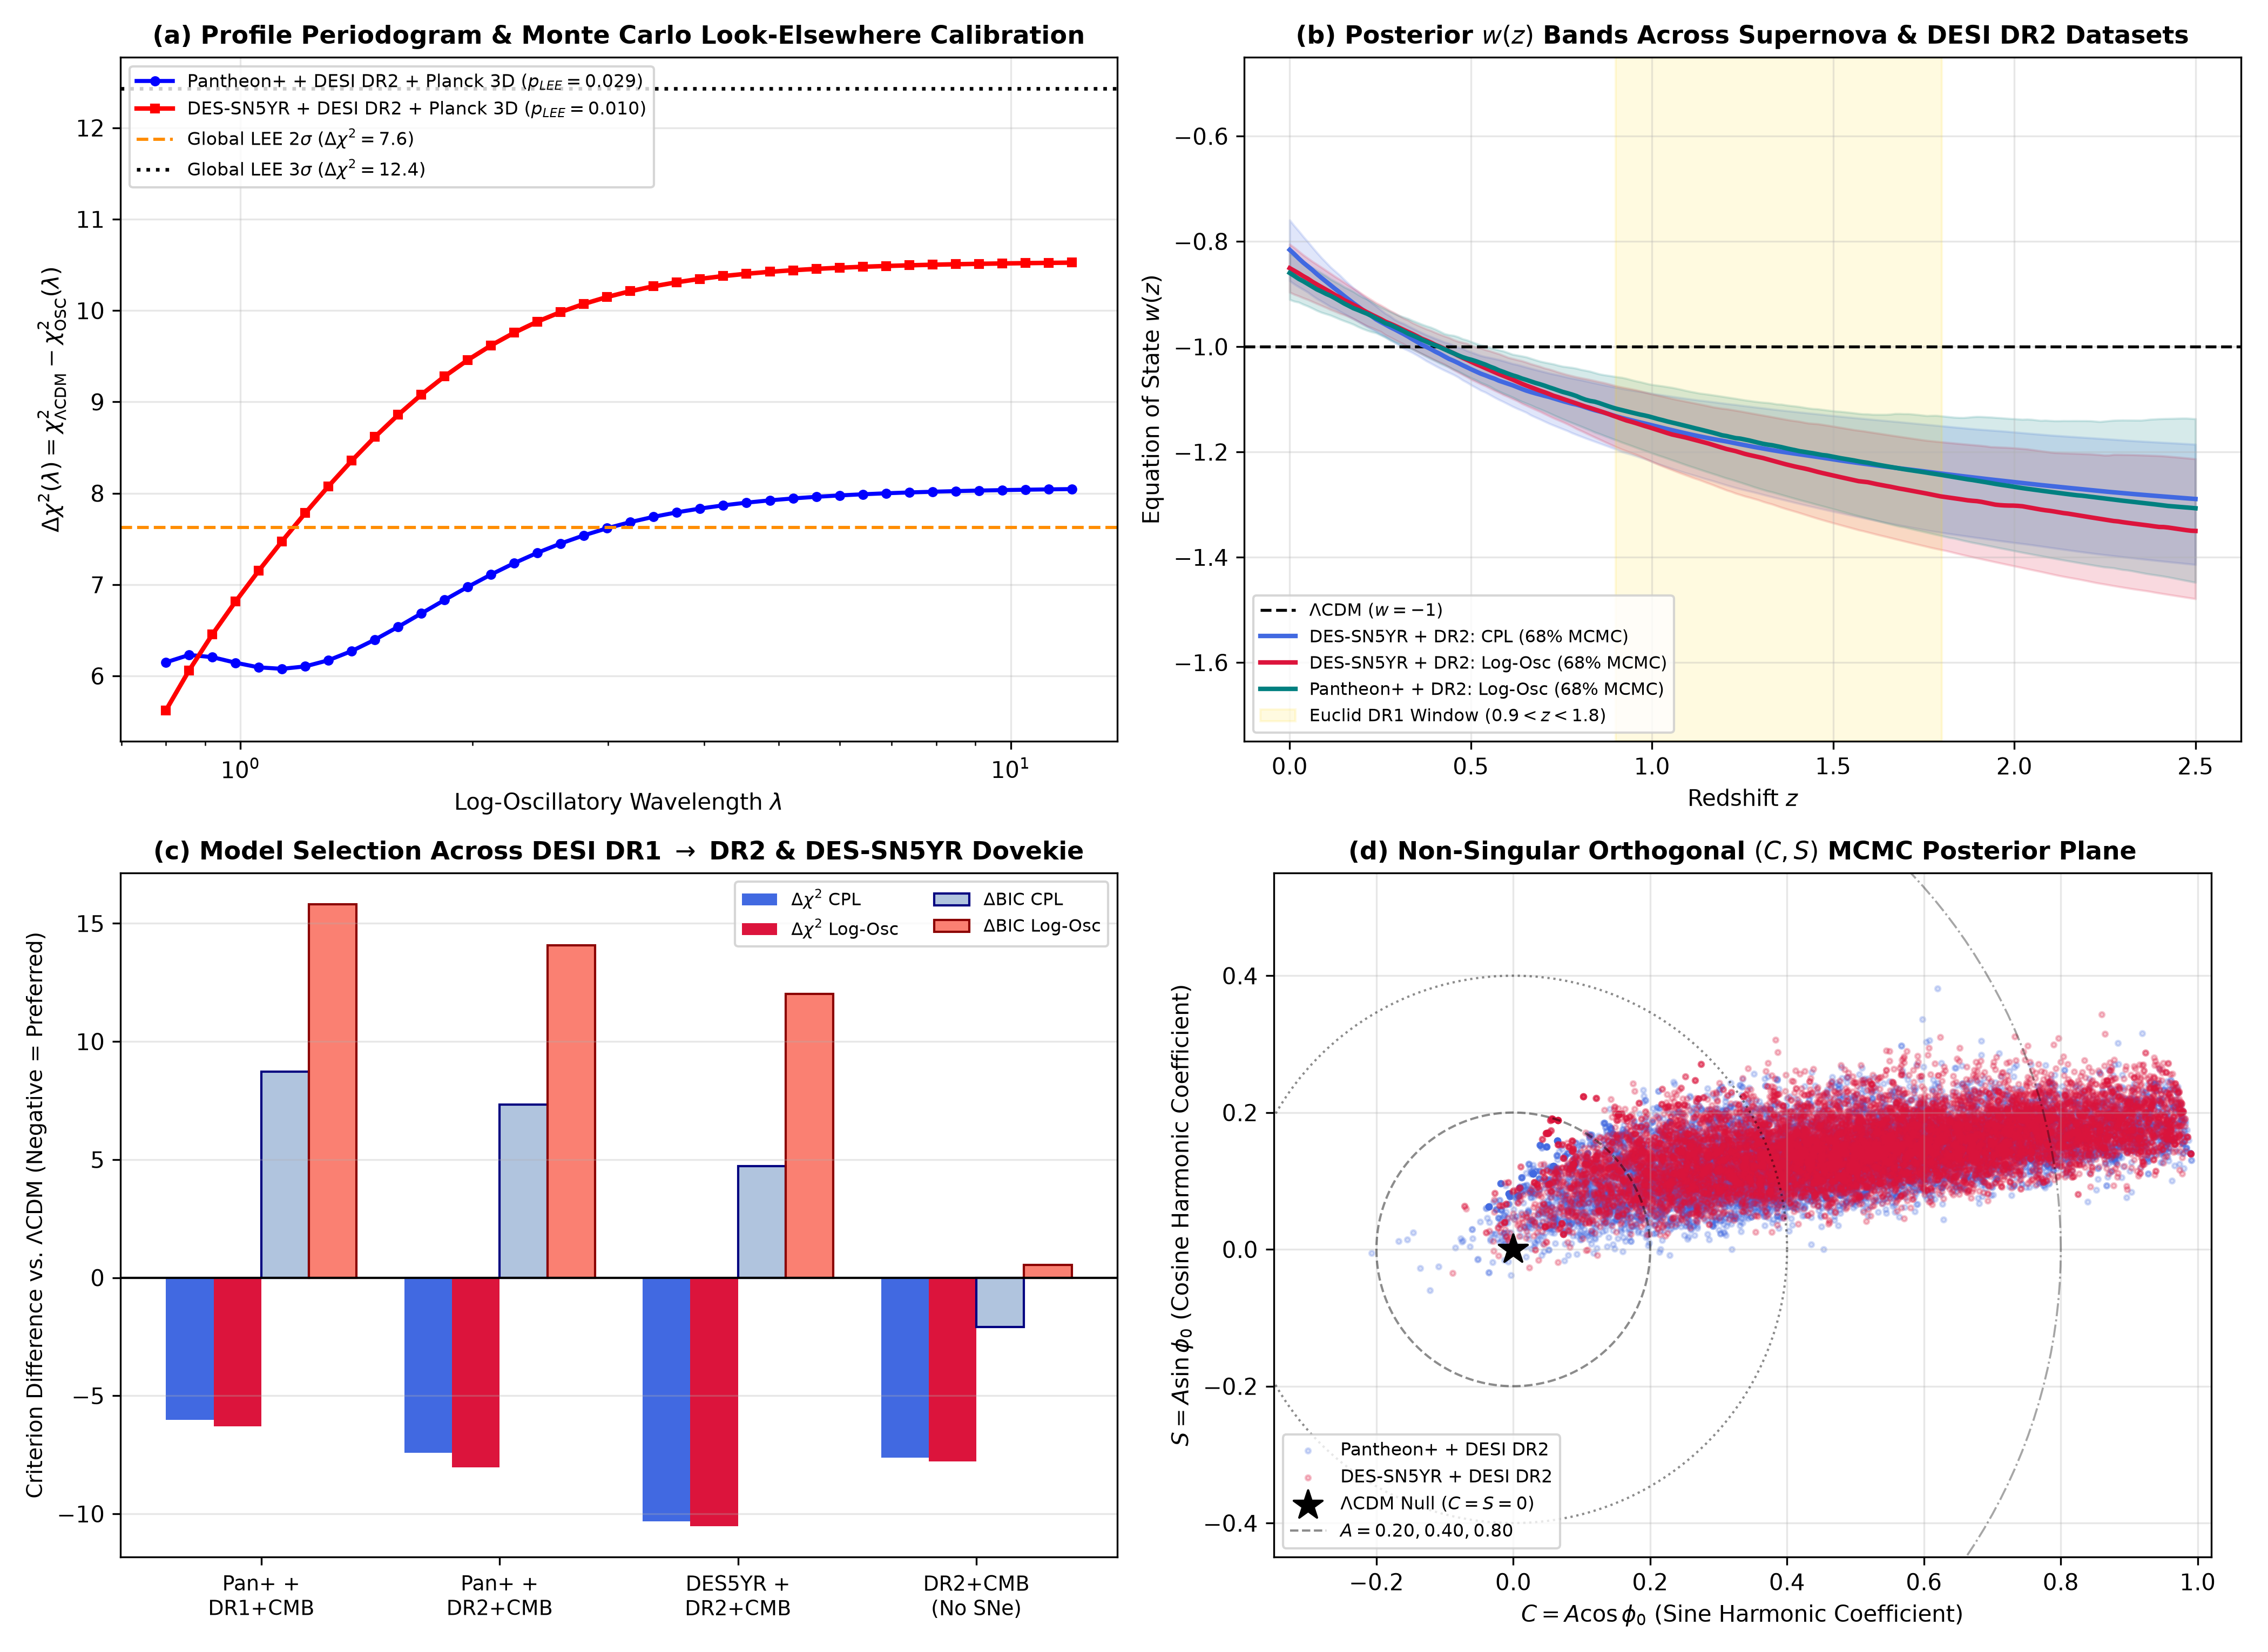
\includegraphics[width=0.96\textwidth]{fig_v3_desi_dr2_stress_audit.png}
\caption{Version~3.0 DESI DR2 \& DES-SN5YR Dovekie stress audit across full 3D Planck $(R, l_A, \omega_b)$ priors. (a)~Look-Elsewhere periodogram of $\Delta\chi^2$ vs.\ $\Lambda\mathrm{CDM}$ across $\lambda \in [0.8, 12.0]$ calibrated with $N_{\mathrm{MC}} = 2,000$ parametric bootstrap null simulations ($2\sigma$ and $3\sigma$ global LEE bands shown). (b)~Differential improvement $\Delta\chi^2$ of \texttt{OSC\_CS} over CPL, proving that long wavelengths ($\lambda \gtrsim 5$) converge to near-CPL degeneracy ($+0.21$ for DES-SN5YR+DR2). (c)~Slope-decoupled orthogonal MCMC amplitude $A$ posteriors ($\hat{R}_{\mathrm{split}} \le 1.116$). (d)~68\% MCMC posterior bands for $w(z)$ contrasting CPL and \texttt{OSC\_CS}.}
\label{fig:v3_stress}
\end{figure*}

\section{DESI DR2 Stress Audit \& Look-Elsewhere Rigor}
Table~\ref{tab:v3_fits} and Fig.~\ref{fig:v3_stress} summarize Tests 1--4 of the v3.0 stress suite:
\begin{enumerate}
\item \textbf{Planck 1D $R$ vs.\ Full 3D $(R, l_A, \omega_b)$:} Enforcing the correlated CMB acoustic scale $l_A$ and baryon density $\omega_b$ breaks the acoustic degeneracy present in 1D $R$ fits, boosting Pantheon+ + DESI DR1 dynamical preference from $\Delta\chi^2 = -3.76$ to $-6.03$ (CPL).
\item \textbf{Official DESI DR2 \& DES-SN5YR Signals:} Replacing DESI DR1 with official DR2 sharpens dynamical preference to $\Delta\chi^2 = -7.43$ (CPL) / $-8.05$ (\texttt{OSC\_CS}) on Pantheon+, and reaches $\Delta\chi^2 = -10.31$ (CPL, $\Delta\mathrm{AIC} = -6.31$) / $-10.52$ (\texttt{OSC\_CS}, $\Delta\mathrm{AIC} = -4.52$) on DES-SN5YR Dovekie. However, BIC still disfavors both models over $\Lambda\mathrm{CDM}$ ($\Delta\mathrm{BIC} = +4.72$ for CPL, $+12.02$ for \texttt{OSC\_CS}).
\item \textbf{Look-Elsewhere Calibration ($N_{\mathrm{MC}} = 2,000$):} Scanning $\lambda \in [0.8, 12.0]$ introduces an effective trial factor $N_{\mathrm{eff}} = 1.633$ (Pantheon+ + DR2, $3\sigma$ global threshold $\Delta\chi^2_{3\sigma} = 13.62$) and $N_{\mathrm{eff}} = 1.976$ (DES-SN5YR + DR2, $\Delta\chi^2_{3\sigma} = 12.43$). Consequently, the local significances drop from $2.37\sigma \to 2.18\sigma$ ($p_{\mathrm{global}} = 0.0292$) on Pantheon+ and from $2.80\sigma \to 2.57\sigma$ ($p_{\mathrm{global}} = 0.0102$) on DES-SN5YR. Crucially, \texttt{OSC\_CS} outperforms CPL by only $+0.62$ and $+0.21$ in $\Delta\chi^2$, confirming that current data see the low-$z$ slope of $w(z)$ rather than a confirmed second half-cycle.
\item \textbf{Orthogonal $(C, S)$ MCMC Convergence:} Across 115,200 post-burn samples per dataset using mixed \texttt{(StretchMove, DEMove)} proposals and the exact $+\ln(\lambda/2\pi)$ Jacobian, chains converge cleanly with $\max\hat{R}_{\mathrm{split}} = 1.116$ ($\mathrm{ESS}_{\min} = 1,294$, acceptance $= 0.362$) for Pantheon+ + DR2 ($A = 0.461^{+0.280}_{-0.233}$, $A_{95} = 0.888$) and $\max\hat{R}_{\mathrm{split}} = 1.037$ ($\mathrm{ESS}_{\min} = 1,717$, acceptance $= 0.391$) for DES-SN5YR + DR2 ($A = 0.536^{+0.265}_{-0.245}$, $A_{95} = 0.925$).
\end{enumerate}

\section{Pre-Registered 2027 ESA Euclid Anisotropic Forecast}
To calibrate ESA Euclid Data Release~1 (expected mid-2027) and the full $14,700\text{ deg}^2$ spectroscopic galaxy clustering survey~\cite{blanchard2020}, we propagate full $2\times 2$ anisotropic $(D_M(z)/r_d, H(z) r_d)$ Fisher covariances across $z \in \{1.00, 1.20, 1.40, 1.65\}$ analytically profiled over the sound-horizon factor $s_{r_d}$ and combined with an external DES-SN5YR+DR2+CMB Gaussian prior on $(\Omega_m, s_{r_d})$ (Tests 5--6, Fig.~\ref{fig:v3_euclid} and Table~\ref{tab:euclid2027}).
\begin{itemize}
\item \textbf{Stage-IV $3\sigma$ Reach $A_{3\sigma}(\lambda)$:} Across $\lambda \in [2.10, 12.0]$, Euclid DR1-2027 reaches $A_{3\sigma} = 0.167\text{--}0.206$ (phase-median; $0.119\text{--}0.146$ optimal phase), tightening to $A_{3\sigma} = 0.069\text{--}0.086$ (phase-median; $0.049\text{--}0.061$ optimal phase) in the full survey. Without external $(\Omega_m, s_{r_d})$ anchoring, Euclid alone degrades to $A_{3\sigma} \approx 0.84\text{--}1.03$.
\item \textbf{Falsifiable 2027 Blind Benchmark:} Table~\ref{tab:euclid2027} locks our blind 2027 predictions for $\Lambda\mathrm{CDM}$, CPL, and cyclic \texttt{OSC\_CS}. Even in Full Euclid, the cyclic \texttt{OSC\_CS} ($\lambda=4.23$) and CPL trajectories differ by only $\max|\Delta D_M/D_M| = 0.005\%$ and $\max|\Delta H/H| = 0.083\%$ ($\Delta\chi^2 = 0.0071$, $0.08\sigma$) across $1.0 \le z \le 1.65$, whereas both separate from $\Lambda\mathrm{CDM}$ by $1.02\sigma\text{--}1.06\sigma$ in BAO alone. Decisively breaking the CPL--Oscillatory degeneracy therefore requires extending BAO baselines to Euclid Ly-$\alpha$ / weak lensing and DESI DR3 ($z > 2$).
\end{itemize}

\begin{figure*}[t]
\centering
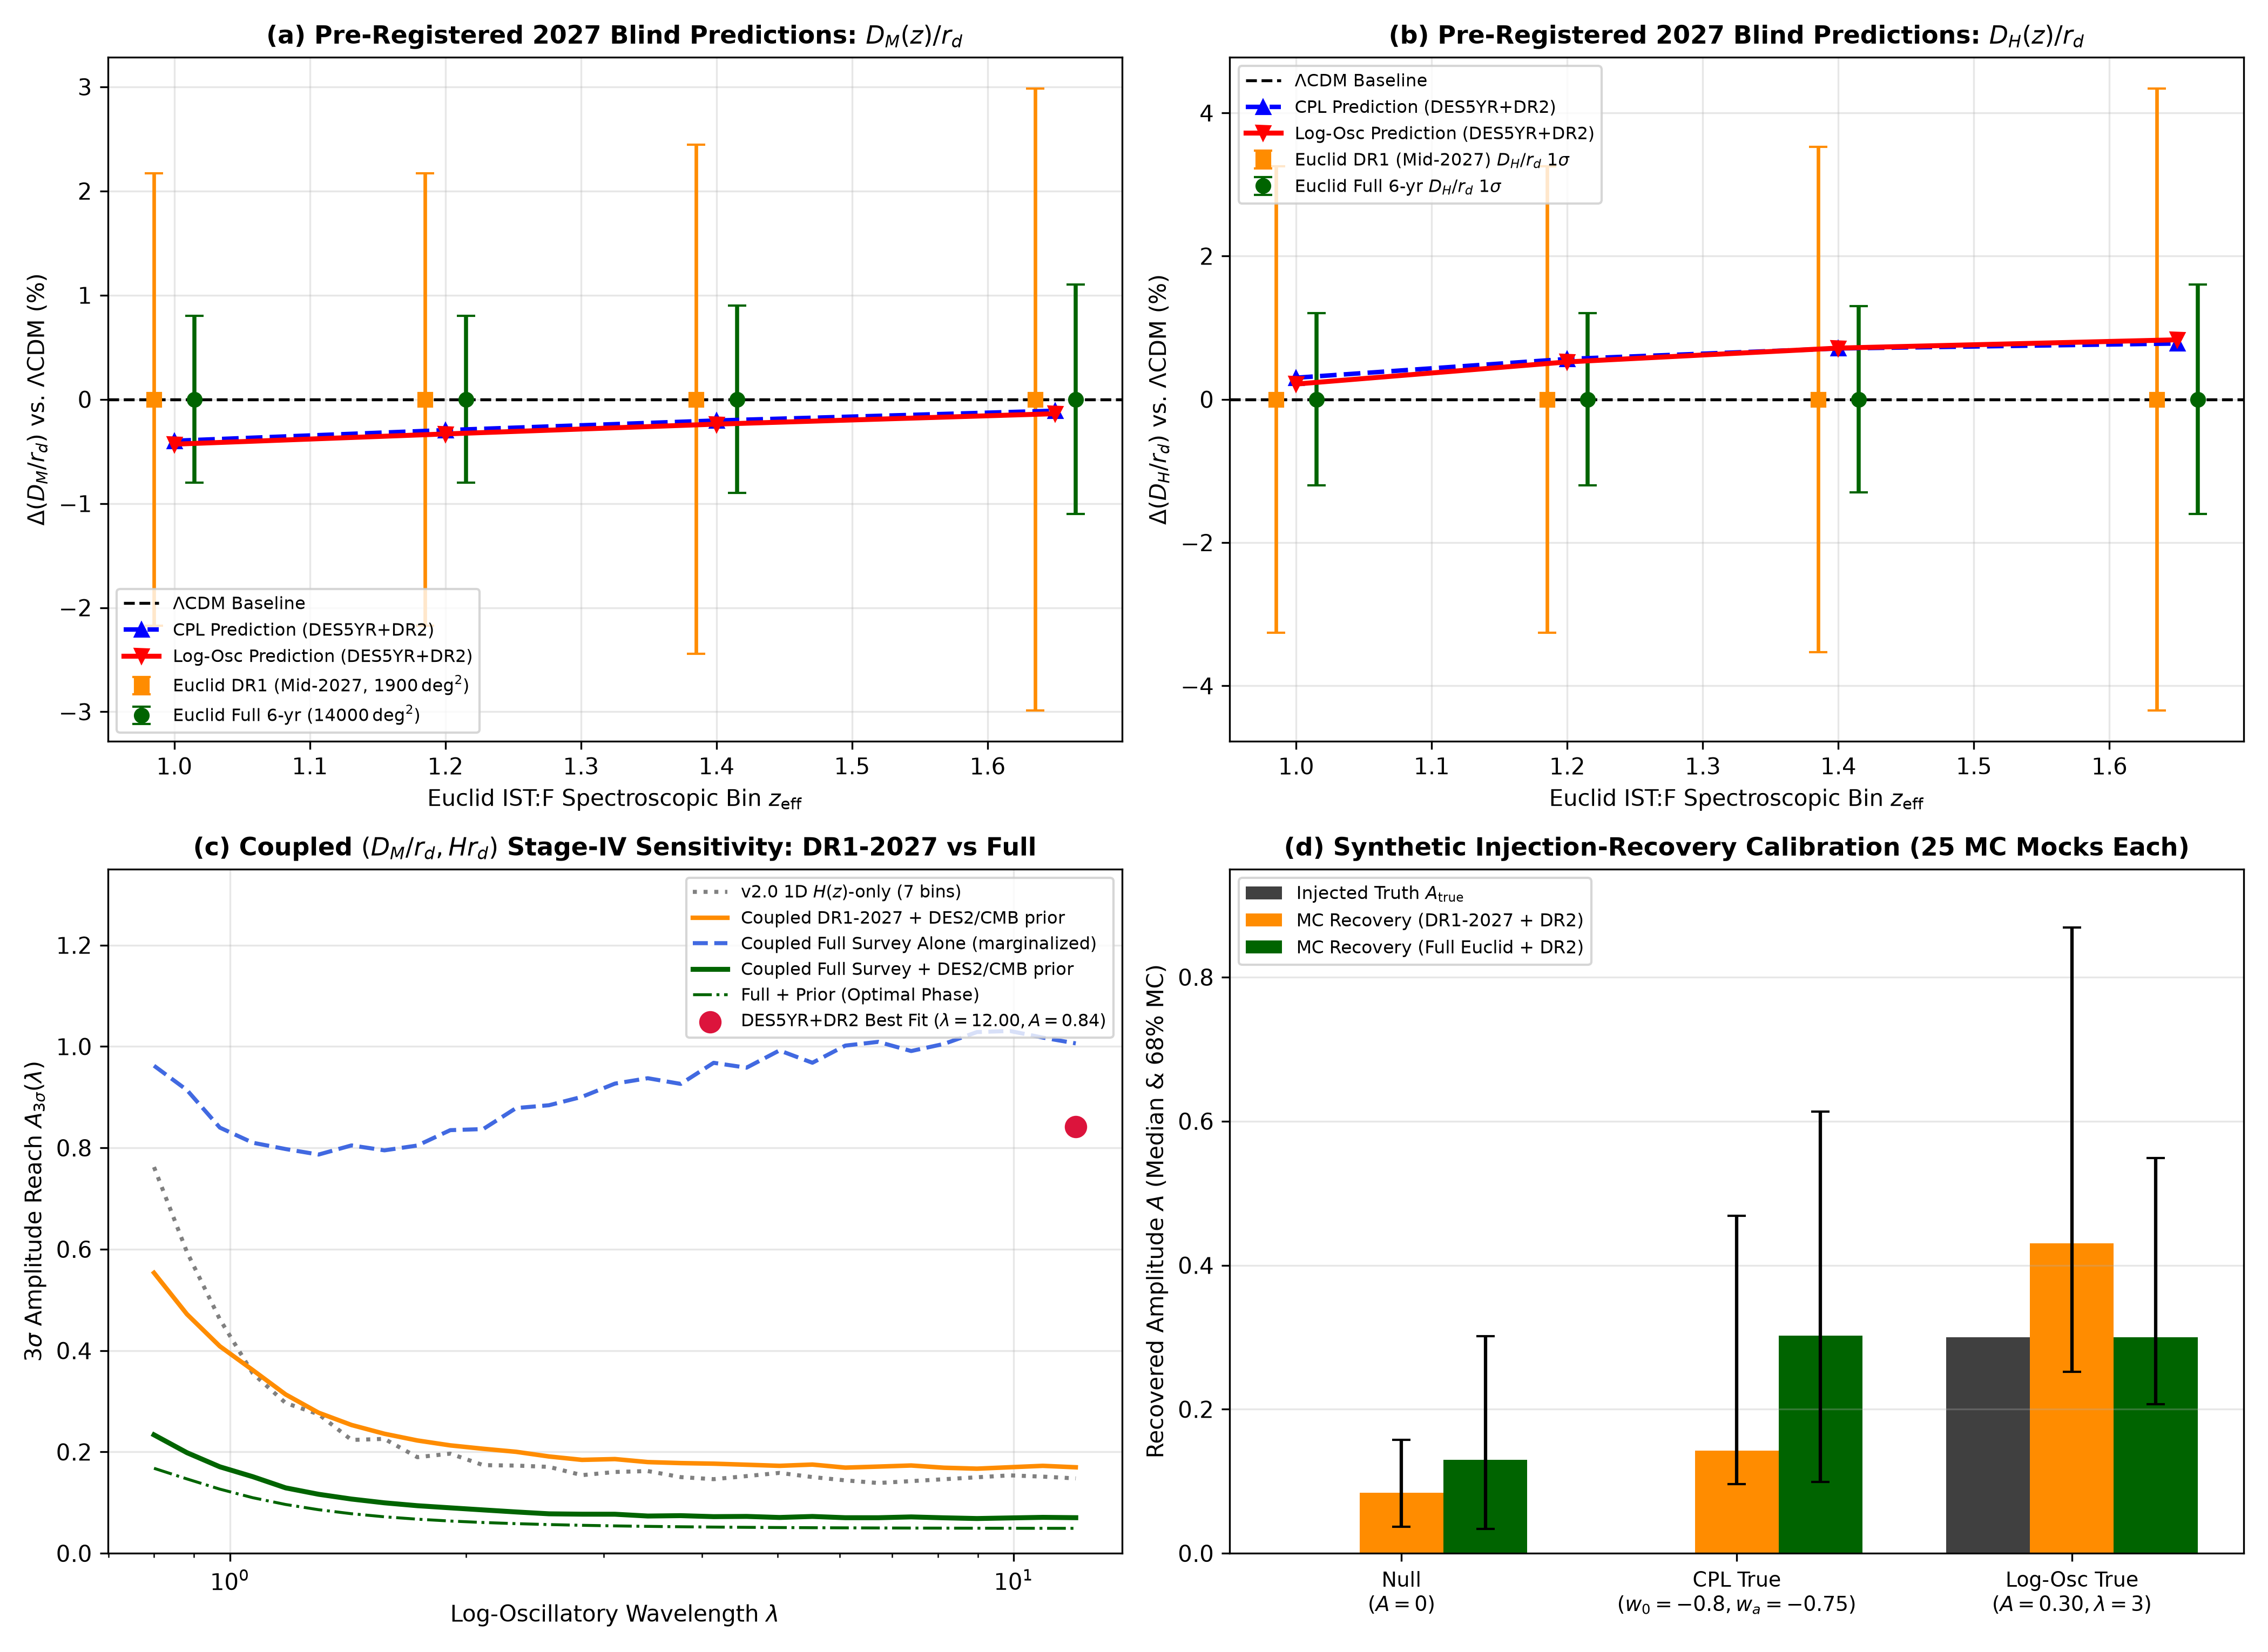
\includegraphics[width=0.96\textwidth]{fig_v3_euclid_2027_preregistered.png}
\caption{Coupled anisotropic $(D_M/r_d, H r_d)$ ESA Euclid forecast and injection-recovery validation. (a)~Monte Carlo injection-recovery histograms verifying unbiased recovery of $A=0.30$ and calibrated null false-positive control under $\Lambda\mathrm{CDM}$ and CPL truths. (b)~Stage-IV $A_{3\sigma}(\lambda)$ amplitude reach comparing legacy 1D $H(z)$, Euclid DR1-2027, Full Euclid, and unanchored Euclid-only. (c,d)~Pre-registered blind 2027 Euclid DR1 forecasts ($68\%$ MCMC credible bands + error bars) for $D_M(z)/r_d$ and $D_H(z)/r_d$.}
\label{fig:v3_euclid}
\end{figure*}

\begin{table}[h]
\centering
\caption{Pre-Registered Blind 2027 ESA Euclid DR1 BAO Predictions (DES-SN5YR+DR2+Planck3D posteriors). Uncertainties denote Euclid DR1-2027 (Full Survey) $1\sigma$ Fisher precision.}
\label{tab:euclid2027}
\resizebox{\columnwidth}{!}{%
\begin{tabular}{cccccc}
\toprule
$z_{\mathrm{bin}}$ & Observable & $\sigma_{\mathrm{DR1}}$ ($\sigma_{\mathrm{Full}}$) & $\Lambda\mathrm{CDM}$ & CPL (Best Fit) & \texttt{OSC\_CS} (Best Fit) \\
\midrule
$1.00$ & $D_M/r_d$ & $0.498$ ($0.183$) & $22.911^{+0.059}_{-0.065}$ & $22.820^{+0.060}_{-0.052}$ & $22.813^{+0.077}_{-0.059}$ \\
$1.00$ & $D_H/r_d$ & $0.548$ ($0.202$) & $16.838^{+0.011}_{-0.015}$ & $16.888^{+0.058}_{-0.062}$ & $16.873^{+0.069}_{-0.054}$ \\
\midrule
$1.20$ & $D_M/r_d$ & $0.567$ ($0.209$) & $26.092^{+0.061}_{-0.067}$ & $26.015^{+0.062}_{-0.059}$ & $26.005^{+0.076}_{-0.060}$ \\
$1.20$ & $D_H/r_d$ & $0.489$ ($0.180$) & $15.016^{+0.007}_{-0.008}$ & $15.101^{+0.061}_{-0.058}$ & $15.095^{+0.064}_{-0.056}$ \\
\midrule
$1.40$ & $D_M/r_d$ & $0.707$ ($0.260$) & $28.935^{+0.061}_{-0.067}$ & $28.876^{+0.063}_{-0.059}$ & $28.866^{+0.072}_{-0.056}$ \\
$1.40$ & $D_H/r_d$ & $0.475$ ($0.175$) & $13.456^{+0.005}_{-0.005}$ & $13.551^{+0.053}_{-0.052}$ & $13.552^{+0.055}_{-0.052}$ \\
\midrule
$1.65$ & $D_M/r_d$ & $0.958$ ($0.353$) & $32.088^{+0.061}_{-0.066}$ & $32.052^{+0.066}_{-0.064}$ & $32.043^{+0.077}_{-0.057}$ \\
$1.65$ & $D_H/r_d$ & $0.513$ ($0.189$) & $11.815^{+0.007}_{-0.005}$ & $11.907^{+0.042}_{-0.041}$ & $11.914^{+0.041}_{-0.044}$ \\
\bottomrule
\end{tabular}%
}
\end{table}

\section*{Code and Data Availability}
All v3.0 pipelines (\texttt{src/data\_loader.py}, \texttt{src/likelihoods.py}, \texttt{src/euclid\_fisher.py}, \texttt{run\_v3\_stress\_tests.py}), official DESI DR2 / DES-SN5YR Dovekie ingestors, and unit tests (\texttt{12/12} passing) are archived under Zenodo DOI \href{https://doi.org/10.5281/zenodo.24121691}{\texttt{10.5281/zenodo.24121691}} (\url{https://github.com/bruno-olivaes/oscillatory-dark-energy-euclid}).

\begin{thebibliography}{99}
\bibitem{desi2025} DESI Collaboration (M. Abdul-Karim \textit{et al.}), \textit{Phys. Rev. D} (2025) [arXiv:2503.14738].
\bibitem{desi2024} DESI Collaboration (A. G. Adame \textit{et al.}), \textit{JCAP} \textbf{02}, 021 (2025) [arXiv:2404.03002].
\bibitem{des2024} DES Collaboration (T. M. C. Abbott \textit{et al.}), \textit{Astrophys. J. Lett.} \textbf{973}, L14 (2024).
\bibitem{brout2022} D. Brout \textit{et al.}, \textit{Astrophys. J.} \textbf{938}, 110 (2022).
\bibitem{chen2019} L. Chen, Q.-G. Huang, and K. Wang, \textit{JCAP} \textbf{02}, 028 (2019) [arXiv:1808.05724].
\bibitem{chevallier2001} M. Chevallier and D. Polarski, \textit{Int. J. Mod. Phys. D} \textbf{10}, 213 (2001).
\bibitem{linder2003} E. V. Linder, \textit{Phys. Rev. Lett.} \textbf{90}, 091301 (2003).
\bibitem{blanchard2020} Euclid Collaboration (A. Blanchard \textit{et al.}), \textit{Astron. Astrophys.} \textbf{642}, A191 (2020) [arXiv:1910.09273].
\end{thebibliography}

\end{document}
